\subsection{PHSD}

Parton-Hadron-String-Dynamics (PHSD)~\cite{PHSD1, PHSD2} is the only model explored in this thesis that utilizes a \textbf{microscopic transport approach}: it simulates the full space-time evolution of a heavy-ion collision by modeling the interactions of individual particles. Here ``particles'' refers to different quantities (strings, partons, hadrons) which are all evolved in different ways. The evolution of a collision within PHSD is as follows.

\subsubsection{Initial stages}
Prior to the collision, the simulation is broken up into a 3D-grid of size 56 in each of the x, y and z directions. The total size of the grid increases with each time step such the number of particles within a given cell evolves smoothly with time. The initial momentum distribution and abundances of partons within the nuclei (prior to any collision) are given by the thermal distributions
\begin{equation}
    f(\omega, \vec{p}) = C_i p^2 \omega \rho_i(\omega, \vec{p}) n_{F / B}(\omega / \tau),
\end{equation}
where $\rho_i$ are the spectral functions of the quarks and gluons ($i = q, \bar{q}, g$) and $n_{F / B}$ are the Fermi-Dirac (for quarks) and Bose-Einstein (for gluons) distributions. Once the nuclei collide, the partons interact with each other under the Lund string model to form \textit{leading hadrons} and \textit{pre-hadrons}, as shown in Figure~\ref{fig:lund_string_phsd}. The leading hadrons are immune to dissociation within the QGP, while the pre-hadrons are not. 

\begin{figure}[ht]
    \centering
    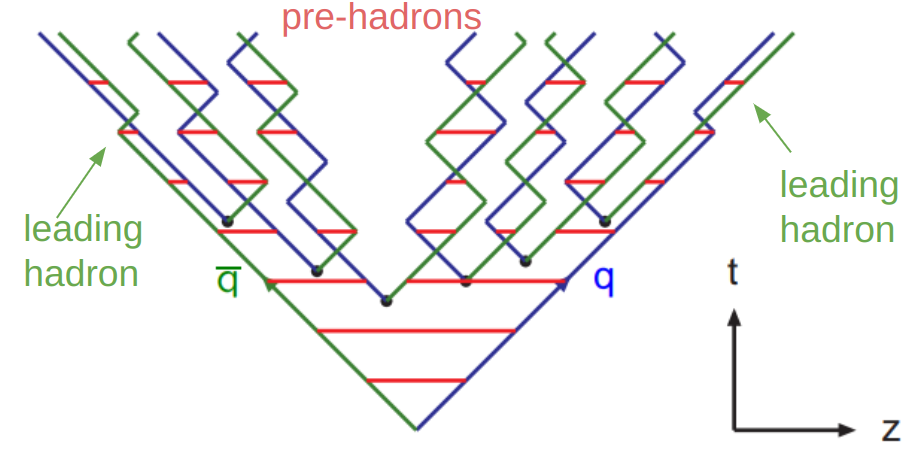
\includegraphics[width=0.5\linewidth]{figures/section_phsd/lund_string_phsd.png}
    \caption{The Lund string model, with pre-hadrons and leading hadrons labeled.}
    \label{fig:lund_string_phsd}
\end{figure}

\subsubsection{QGP phase}




